\documentclass[a4paper,
fontsize=11pt,
%headings=small,
oneside,
numbers=noperiodatend,
parskip=half-,
bibliography=totoc,
final
]{scrartcl}

\usepackage[babel]{csquotes}
\usepackage{synttree}
\usepackage{graphicx}
\setkeys{Gin}{width=.4\textwidth} %default pics size

\graphicspath{{./plots/}}
\usepackage[english]{babel}
\usepackage[T1]{fontenc}
%\usepackage{amsmath}
\usepackage[utf8x]{inputenc}
\usepackage [hyphens]{url}
\usepackage{booktabs} 
\usepackage[left=2.4cm,right=2.4cm,top=2.3cm,bottom=2cm,includeheadfoot]{geometry}
\usepackage[labelformat=empty]{caption} % option 'labelformat=empty]' to surpress adding "Abbildung 1:" or "Figure 1" before each caption / use parameter '\captionsetup{labelformat=empty}' instead to change this for just one caption
\usepackage{eurosym}
\usepackage{multirow}
\usepackage[ngerman]{varioref}
\setcapindent{1em}
\renewcommand{\labelitemi}{--}
\usepackage{paralist}
\usepackage{pdfpages}
\usepackage{lscape}
\usepackage{float}
\usepackage{acronym}
\usepackage{eurosym}
\usepackage{longtable,lscape}
\usepackage{mathpazo}
\usepackage[normalem]{ulem} %emphasize weiterhin kursiv
\usepackage[flushmargin,ragged]{footmisc} % left align footnote
\usepackage{ccicons} 
\setcapindent{0pt} % no indentation in captions
\usepackage{xurl} % Breaks URLs

%%%% fancy LIBREAS URL color 
\usepackage{xcolor}
\definecolor{libreas}{RGB}{112,0,0}

\usepackage{listings}

\urlstyle{same}  % don't use monospace font for urls

\usepackage[fleqn]{amsmath}

%adjust fontsize for part

\usepackage{sectsty}
\partfont{\large}

%Das BibTeX-Zeichen mit \BibTeX setzen:
\def\symbol#1{\char #1\relax}
\def\bsl{{\tt\symbol{'134}}}
\def\BibTeX{{\rm B\kern-.05em{\sc i\kern-.025em b}\kern-.08em
    T\kern-.1667em\lower.7ex\hbox{E}\kern-.125emX}}

\usepackage{fancyhdr}
\fancyhf{}
\pagestyle{fancyplain}
\fancyhead[R]{\thepage}

% make sure bookmarks are created eventough sections are not numbered!
% uncommend if sections are numbered (bookmarks created by default)
\makeatletter
\renewcommand\@seccntformat[1]{}
\makeatother

% typo setup
\clubpenalty = 10000
\widowpenalty = 10000
\displaywidowpenalty = 10000

\usepackage{hyperxmp}
\usepackage[colorlinks, linkcolor=black,citecolor=black, urlcolor=libreas,
breaklinks= true,bookmarks=true,bookmarksopen=true]{hyperref}
\usepackage{breakurl}

%meta
%meta

\fancyhead[L]{A. Abalkina\\ %author
LIBREAS. Library Ideas, 47 (2025). % journal, issue, volume.
\href{https://doi.org/10.18452/x}{\color{black}https://doi.org/10.18452/x}
{}} % doi 
\fancyhead[R]{\thepage} %page number
\fancyfoot[L] {\ccLogo \ccAttribution\ \href{https://creativecommons.org/licenses/by/4.0/}{\color{black}Creative Commons BY 4.0}}  %licence
\fancyfoot[R] {ISSN: 1860-7950}

\title{\LARGE{Journal hijacking: challenges for the scientific community and recommendations for journals}}% title
\author{Anna Abalkina} % author

\setcounter{page}{1}

\hypersetup{%
      pdftitle={Journal hijacking: challenges for the scientific community and recommendations for journals},
      pdfauthor={Anna Abalkina},
      pdfsubject={LIBREAS. Library Ideas, 47 (2025)},
      pdfkeywords={scholarly publishing, fraud, journal, hijacking},
      pdflicenseurl={https://creativecommons.org/licenses/by/4.0/},
      pdfcopyright={CC BY 4.0 International},
      pdfcontacturl={http://libreas.eu},
      pdfurl={},
      pdfdoi={},
      pdflang={en},
      pdfmetalang={en}
     }


\date{}
\begin{document}

\maketitle
\thispagestyle{fancyplain} 

%abstracts

%body
Hijacked journals (also known as cloned journals) are a type of
cybercrime. They copy the title, ISSN, and other metadata of legitimate
journals and claim to be the authentic journal in order to attract
authors and publish their papers in exchange for article processing
charges (Abalkina, 2021; Jalalian \& Dadkhah, 2015; Moussa, 2021). This
phenomenon was first documented around 2011 (Jalalian \& Dadkhah, 2015).
Since then, hundreds of journals have been hijacked.

There are two methods of journal hijacking. First, fraudulent publishers
create an alternative website for an existing journal, claiming that it
is the genuine one (see Figure 1). This type of hijacking can be
successful because they target print-only journals, and the fake website
becomes the only visible online presence of the journal. They also clone
journals published in local languages. This strategy has been especially
effective with Chinese journals.

\pagebreak

\textbf{Figure 1: \emph{Chinese Journal of Evidence-Based Medicine}:
authentic and cloned websites}

\begin{figure}[H]
\centering
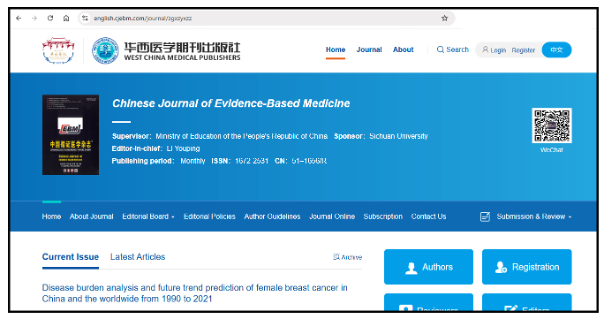
\includegraphics[width=.7\textwidth]{img/fig1a.png}
\caption{Fig. 1a: Authentic journal (Source: \url{https://www.cjebm.net/})}
\end{figure}

\begin{figure}[H]
\centering
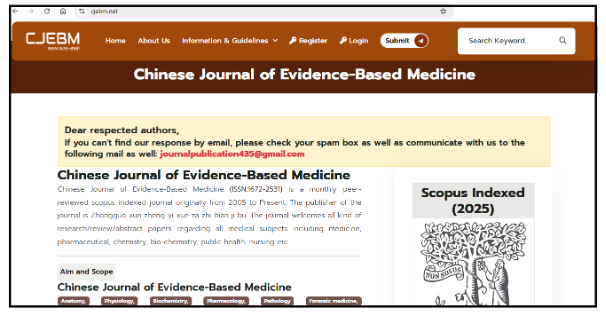
\includegraphics[width=.7\textwidth]{img/fig1b.png}
\caption{Fig. 1b: Hijacked journal (Source: \url{https://web.archive.org/web/20190331173644/https://www.russianlawjournal.org/jour})}
\end{figure}

Another method is to register the expired web domain of an existing
journal (Bohannon, 2015). This can happen when a journal ceases
publication or when the original publisher fails to renew the domain
registration. For example, the \emph{Russian Law Journal} ceased
publication, a fraudulent publisher registered its expired domain and
created a journal website of the \emph{Russian Law Journal} and accepted
hundreds of papers in different disciplines, which were subsequently
indexed in Web of Science (Abalkina, 2023b) (see Figure 2).

\pagebreak

\textbf{Figure 2: \emph{Russian Law Journal}: authentic and hijacked
websites}

\begin{figure}[H]
\centering
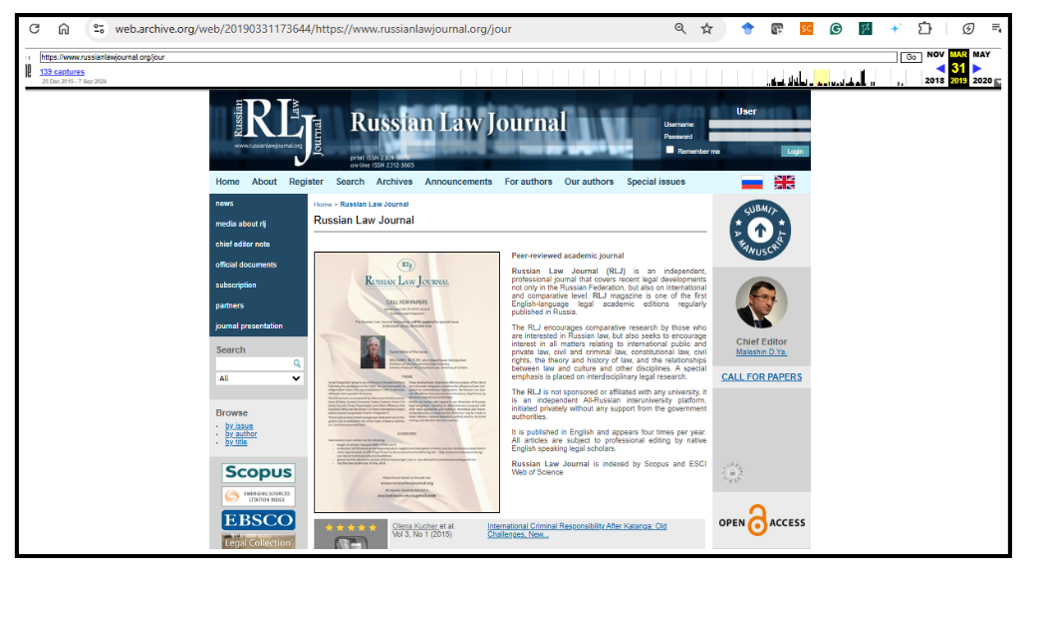
\includegraphics[width=.7\textwidth]{img/fig2a.png}
\caption{Fig. 2a: Authentic journal (2019) (Source: \url{https://web.archive.org/web/20190331173644/https://www.russianlawjournal.org/jour})}
\end{figure}

\begin{figure}[H]
\centering
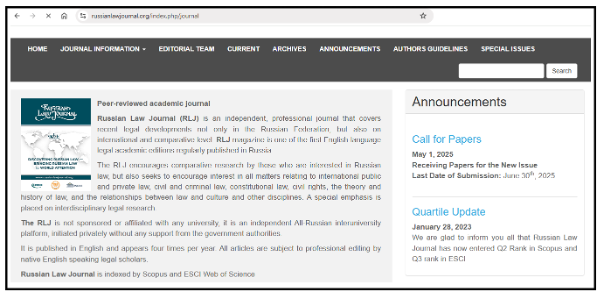
\includegraphics[width=.7\textwidth]{img/fig2b.png}
\caption{Fig. 2b: Hijacked journal (2025) (Source: \url{https://www.russianlawjournal.org/index.php/journal})}
\end{figure}

More than 400 cases of hijacked journals have been documented since 2012
across different lists. The first list was created by the US-American
librarian Jeffrey Beall, but he stopped updating it in 2017. Cabell's, a
paywalled database of journals, also includes hijacked journals as part
of its criteria in \emph{Predatory Reports}, which evaluates journals
based on deceptive, fraudulent, or predatory practices. Another list has
been compiled by UGC CARE in India\footnote{The Indian University Grants
  Commission (UGC) first introduced the UGC Consortium for Academic and
  Research Ethics (UGC-CARE) list in 2018, listing quality academic
  journals.}, which includes Cloned List I for local hijacked journals
and Cloned List II for those indexed in international databases.
However, UGC CARE is discontinuing its journal list used for research
evaluation purposes (The Economic Times, 2025). It is unclear whether
the lists of cloned journals will continue to be updated. Another list
is the Retraction Watch Hijacked Journal Checker\footnote{Retraction
  Watch Hijacked Journal Checker:
  \url{https://retractionwatch.com/the-retraction-watch-hijacked-journal-checker/}},
created in May 2022 and regularly updated. As of May 2025, the list
includes more than 350 entries of hijacked journals.

The majority of original journals have been hijacked once, though some
are associated with two cloned websites. The case of the Seybold Journal
is notable, with five cloned websites (Abalkina, 2023a). Such multiple
cloning of journals by different fraudulent publishers can be explained
by the fact that certain types of legitimate journals are particularly
targeted, for example, trade journals, small, niche and print-only
journals, or journals published in local languages (Jalalian \&
Mahboobi,~2014; Shahri et al.,~2018). Hijackers normally don't clone
journals by major publishers, though individual cases have been
reported. For instance, in 2024 a fraudulent publisher cloned 13
journals published by Elsevier, Springer, etc. (Abalkina, 2024a). A
striking detail is that the cloned webpages were identical to the
authentic journals, the only difference was the web domain address,
which was slightly different from the original.

Hijacked journals are not as numerous as predatory journals, but their
proliferation also poses a significant challenge to the scientific
community. They threaten scientific integrity by offering rapid
publication without peer review, distorting international database
indexes, and serving as repositories for low-quality papers and research
involving misconduct. Such papers are nonetheless cited in reputable
journals and indexed in various bibliographic databases.

There is evidence that unreviewed papers published in hijacked journals
can be indexed in Scopus or Web of Science. A study by Abalkina (2024b)
identified 67 hijacked journals that have penetrated Scopus since 2013,
of which 33 have indexed unauthorized content, 23 compromised the
journal's homepage link in Scopus, and 11 did both. There is also
evidence of hijacked journals penetrating Web of Science (Abalkina,
2023b; Butler, 2013). Hijacked journals are indexed in Google Scholar as
well, and scholars should be cautious when retrieving data or conducting
literature searches through this platform.

\section{Features of hijacked
journals}\label{features-of-hijacked-journals}

Hijacked journals present themselves as multidisciplinary journals. The
topics of the papers they accept are usually from various disciplines
and often do not correspond to the title of the journal. This happens
because hijacked journals aim to accept as many papers as possible to
maximize their profit. Low article processing charges (APCs) are another
potential \enquote{red flag} of a fraudulent journal. Bhasker and
Solomon (2025) note that low APCs of \$25 per article are a specific
diagnostic indicator of pseudo-journals. Such low fees can be explained
by the limited payment capacity in countries where most authors
publishing in hijacked journals are based, for example India, Indonesia,
Uzbekistan, etc.

Hijacked journals publish papers within a matter of days, which is
problematic because a genuine publication process requires both
editorial assessment of the manuscript and a peer review process, both
of which take time.

Hijacked journals may assign fake DOIs starting with numbers such as 12,
16 or 20 (see Figure~3), although a legitimate DOI always begins with
10. Sometimes, fraudulent publishers register real DOIs for hijacked
journals. In such cases, it is possible to identify that the publisher
is not the original one by cross-checking the information in the ISSN
Portal or Crossref.

\textbf{Figure 3: A cloned version of gis.Science: Die Zeitschrift für
Geoinformatik}

\begin{figure}[H]
\centering
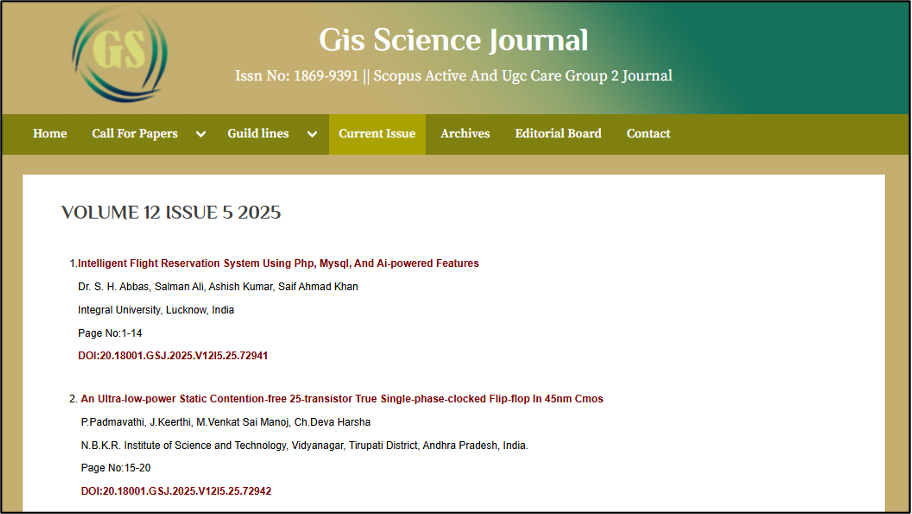
\includegraphics[width=.7\textwidth]{img/fig3.png}
\caption{Fig. 3: Hijacked journal (Source: \url{https://gisscience.net/volume-12-issue-5-2025/})}
\end{figure}

Some hijacked journals provide fake editorial boards or copy them from
other journals. They may also present fabricated journal metrics and
incorrect impact factor values (Dadkhah et al., 2016) and claim
indexation in different bibliographic databases, such as Scopus or Web
of Science.

One of the red flags of hijacked journals is an anonymously registered
and recently created domain, which can be verified using a WHOIS
service. A recent registration makes it difficult for a hijacked journal
to demonstrate a history of regular publication or the availability of
an archive, which potential authors expect to see in a legitimate
journal. For this reason, hijacked journals may create a fake archive
filled with articles copied from other hijacked journals or generated by
AI (Abalkina, 2021). Often the texts of these archived papers are not
accessible due to paywall, likely because they do not exist. However, an
archive is an important feature of a journal, as it indicates the
continuous publication of journal issues (Dony et al., 2020).

\section{What Can Be Done? Recommendations for
Journals}\label{what-can-be-done-recommendations-for-journals}

Authentic journals that are hijacked face several challenges. They
experience an increased editorial workload due to letters from authors
who have fallen victim to the hijacked versions. Editors must take
additional measures to prevent further damage to the journal, neutralize
the hijacked version, and take steps to restore accurate information in
bibliographic databases if the hijacked journal has led to the indexing
of unauthorized content. Müller \& Sæbø (2023) discuss such challenges
in the case of the hijacking of their journal, \emph{Scandinavian
Journal of Information Systems}.

These challenges highlight the need for a proactive response from
journals and editors in case of hijacking. The following measures can
help journals to prevent hijacking, protect the journal and potential
authors, as well as mitigate the negative effects caused by hijacking:

\begin{itemize}
\item
  Ensure the security of the journal\textquotesingle s website and renew
  the domain registration in a timely manner. Passwords and access
  credentials should be stored securely. It is also important to plan
  for situations in which a colleague who holds the access credentials
  leaves the job and there should always be an alternative means of
  access to data storage. There have been cases where journals lost
  their web domains because they were unable to regain access.
\item
  Journals should improve their search engine optimization (SEO), as
  hijacked journals actively promote fraudulent websites that often
  appear among the top search results in different search engines.
\end{itemize}

In case of hijacking:

\begin{itemize}
\item
  Submit a complaint to the domain registrar and hosting provider.
  Provide all available evidence of the illegitimate use of the
  journal's title, ISSN, and other metadata. Include the details of the
  hijacked journal and any known contact information.
\item
  You may consider contacting Visa, MasterCard, PayPal, etc., to disrupt
  the payment process of the hijacked journal if it is receiving
  payments for publications.
\item
  Publish information about the journal hijacking on the homepage of the
  legitimate journal\textquotesingle s website to inform authors about
  the fraudulent site. If the website is in a language other than
  English, consider adding the message in English as well, since the
  main victims of journal hijacking are often authors from East, South,
  and Central Asia.
\item
  Inform the Retraction Watch Hijacked Journal Checker about the
  hijacking case by filling out the form\footnote{Retraction Watch
    Hijacked Journal Checker form:
    \url{https://docs.google.com/forms/d/e/1FAIpQLScOZ6qj8ZwpkGh8IH7Z43xnxgY8B9wPHUKXnK50ikVv3HC-Dg/viewform}}.
  Please also indicate the original website. If the case is confirmed,
  the database will be updated accordingly.
\item
  If the journal has lost its web domain, inform indexing databases (e.\,g., Scopus, Web of Science, Scimago, DOAJ) about the case. Fraudulent
  publishers may use the domain to host a fake journal and index
  unreviewed papers in various bibliographic databases.
\item
  Fraudulent publishers may also register a new DOI prefix for the
  hijacked journal. This can be checked via the Crossref title
  list\footnote{Crossref title list:
    \url{https://www.crossref.org/titleList/}}. If this has occurred,
  provide all available evidence of hijacking to Crossref. This may lead
  to the exclusion of the member from Crossref like in the case of a
  suspicious \enquote{Springer Global Publications} which had cloned the
  website of journals published by Springer, Elsevier, and other major
  publishers (Kincaid, 2024).
\end{itemize}

\section{Conclusions}\label{conclusions}

Hijacked journals are a type of fraudulent journal that poses a
significant challenge to academic publishing by exploiting the
reputation of legitimate journals. The proliferation of hijacked
journals highlights vulnerabilities in the scholarly communication
infrastructure, insufficient verification processes in indexing
databases, limited awareness of the problem, and the use of publications
in hijacked journals for research evaluation.

Tackling the problem of hijacked journals requires a coordinated and
proactive response from multiple stakeholders. This includes stronger
verification and response mechanisms from indexing databases, increased
awareness of the issue, educating scholars on how to recognize hijacked
journals to avoid submitting papers to or citing from them, and
preventive actions by legitimate journals to protect themselves from
being hijacked.

\section{Conflict of interest}\label{conflict-of-interest}

Anna Abalkina is a co-founder of the Retraction Watch Hijacked Journal
Checker.

\section{References}\label{references}

Abalkina, A. (2021). Detecting a network of hijacked journals by its
archive. Scientometrics, 126, 7123--7148.
\url{https://doi.org/10.1007/s11192-021-04056-0}.

Abalkina, A. (2023a). How many times can a journal be hijacked?
Retraction Watch, 24 February 2023.
\url{https://retractionwatch.com/2023/02/24/how-many-times-can-a-journal-be-hijacked/}.

Abalkina, A. (2023b). Three journals' web domains expired. Then major
indexes pointed to hijacked versions. Retraction Watch, 26 May 2023.
\url{https://retractionwatch.com/2023/05/26/three-journals-web-domains-expired-then-major-indexes-pointed-to-hijacked-versions/}.

Abalkina, A. (2024a). New hijacking scam targets Elsevier, Springer
Nature, and other major publishers. Retraction Watch, 25 November 2024.
\url{https://retractionwatch.com/2024/11/25/exclusive-new-hijacking-scam-targets-elsevier-springer-nature-and-other-major-publishers/}.

Abalkina, A. (2024b). Challenges posed by hijacked journals in Scopus.
Journal of the Association for Information Science and Technology,
75(4), 395--422. \url{https://doi.org/10.1002/asi.24855}.

Bhasker, J., \& Vijay Solomon, R. (2025). The cost of deception:
pseudo-journals and exploitative article processing charges. Research
Evaluation, 34, rvaf017. \url{https://doi.org/10.1093/reseval/rvaf017}.

Bohannon, J. (2015). How to hijack a journal. Science, 350(6263),
903--905. \url{https://doi.org/10.1126/science.aad7463}.

Butler, D. (2013). Sham journals scam authors. Nature, 495, 421--422.
\url{https://doi.org/10.1038/495421a}.

Dadkhah, M., Maliszewski, T., \& Teixeira da Silva, J. A. (2016).
Hijacked journals, hijacked web-sites, journal phishing, misleading
metrics, and predatory publishing: Actual and potential threats to
academic integrity and publishing ethics. Forensic Science, Medicine,
and Pathology, 12, 353--362.
\url{https://doi.org/10.1007/s12024-016-9785-x}.

Dony, C., Raskinet, M., Renaville, F., Simon, S., Thirion, P. (2020).
How reliable and useful is Cabell's blacklist? A Data-Driven Analysis.
LIBER Quarterly, 30, 1--38. \url{https://doi.org/10.18352/lq.10339}.

Jalalian, M., \& Dadkhah, M. (2015). The full story of 90 hijacked
journals from August 2011 to June 2015. Geographica Pannonica, 19(2),
73--87. \url{https://doi.org/10.18421/GP19.02-06}.

Jalalian, M., \& Mahboobi, J. (2014). Hijacked journals and predatory
publishers Is there a need to re-think how to assess the quality of
academic research. Walailak Journal of Science and Technology, 11(5),
389--394. \url{https://doi.org/10.14456/WJST.2014.16}.

Kincaid, E. (2024). Crossref suspends company's membership after
Retraction Watch report. Retraction Watch. 2 December 2024.
\url{https://retractionwatch.com/2024/12/02/crossref-suspends-companys-membership-after-retraction-watch-report/}.

Moussa, S. (2021b). Journal hijacking: Challenges and potential
solutions. Learned Publishing, 34(4), 688--695.
\url{https://doi.org/10.1002/leap.1412}.

Müller, S. D., \& Sæbø, J. I. (2023). The \enquote{hijacking} of the
Scandinavian Journal of Information Systems: Implications for the
information systems community. Information Systems Journal, 2023, 1--20.
\url{https://doi.org/10.1111/isj.12481}.

Shahri, et al.~(2018). Detecting Hijacked journals by using
classification algorithms. Science and Engineering Ethics, 24, 655--668.
\url{https://doi.org/10.1007/s11948-017-9914-2}.

The Economic Times. (2025). UGC discontinues CARE List journals,
switches to decentralised journal evaluation. The Economic Times, 11
February 2025.
\url{https://economictimes.indiatimes.com/industry/services/education/ugc-discontinues-care-list-journals-switches-to-decentralised-journal-evaluation/articleshow/118150336.cms?from=mdr}.

%autor
\begin{center}\rule{0.5\linewidth}{0.5pt}\end{center}

\textbf{Dr.~Anna Abalkina} (\url{https://orcid.org/0000-0003-1469-4907})
is a research fellow at Freie Universität Berlin specialized in academic
corruption, including plagiarism, paper mills, and hijacked journals.
Originally trained in international economics, she shifted her focus to
investigating scientific misconduct and its systemic consequences. Since
2013, she has collaborated with Dissernet to expose academic fraud in
Russia and has identified over 1,000 suspicious papers linked to
fraudulent publishing practices. She co-developed the ``Retraction Watch
Hijacked Journal Checker'' to help researchers detect scam journals. In
recognition of her impact, Nature named her one of ten people who shaped
science in 2024.

\end{document}